\documentclass[11pt,a4paper]{article}
\usepackage[utf8]{inputenc}
\usepackage[english]{babel}
 
\usepackage{graphicx}
\usepackage{listings}
\usepackage{graphics}
\usepackage[T1]{fontenc}
\usepackage[margin=1.2in]{geometry}
\usepackage{tcolorbox}
\usepackage{hyperref}
\usepackage{dingbat}
\usepackage{float}
\usepackage{tocloft}

\begin{document}
\begin{titlepage}
\title{Bluetooth Low Energy (BLE)}
\author{e-Yantra Team}
\date{\today}
\maketitle
\end{titlepage}

    \listoffigures
    \tableofcontents
    \newpage
    
    	\section{ Introduction to BLE}
    	\subsection{What is BLE ?}
    	\begin{figure}[h]
\centering
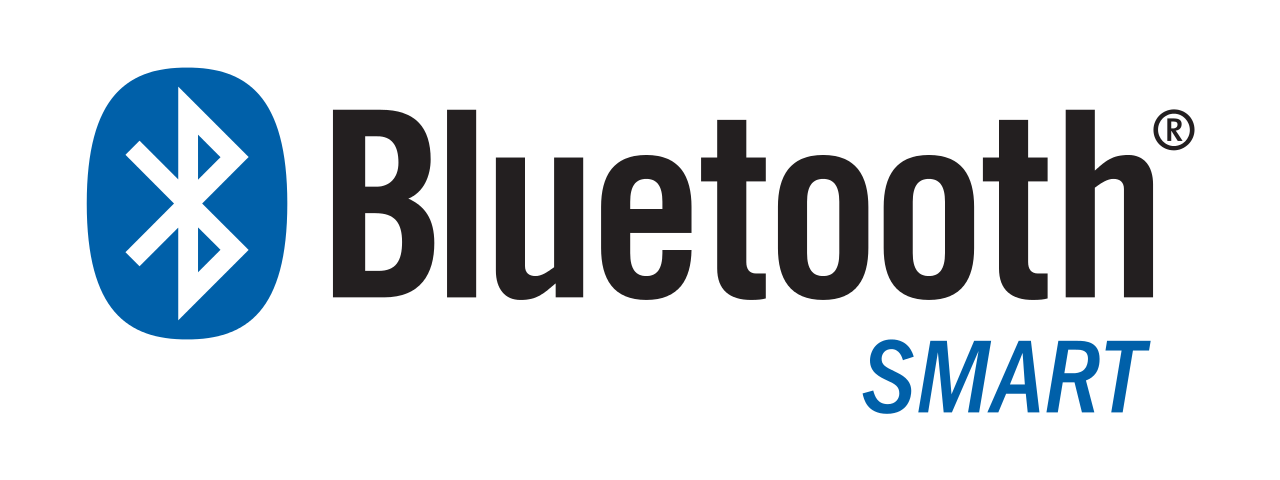
\includegraphics[width=8cm,height=4cm]{Bluetooth_Smart_Logo.png}
\caption{Bluetooth Smart Logo}
\end{figure}
	 { BLE is a wireless personal area network technology designed and marketed by the Bluetooth Special Interest Group aimed at novel applications in the healthcare, fitness, beacons, security, and home entertainment industries. Bluetooth Low Energy (often referred to as Bluetooth LE, BLE, or Bluetooth Smart) takes the same Bluetooth technology used in our cars and mobile devices and allows it to constantly run and collect data use very little energy. 
	 
 Bluetooth Smart Low Energy allows devices like toys, wearables, and appliances to function for months at a time without needing more than the standard coin cell batteries. Bluetooth LE is often used for devices that fall into the Internet of Things (IoT) categories, using efficient low energy to power sensors in pedometers, glucose monitors, security devices and features, smartphones and computers, and much more. BLE devices use much less power than standard Bluetooth connections, while still offering close to the same Bluetooth connectivity at about one-half of its range. 
 
 It is an emerging low-power wireless technology developed for short-range control and monitoring applications that is expected to be incorporated into billions of devices in the next few years. This paper describes the main features of BLE, explores its potential applications, and investigates the impact of various critical parameters on its performance. BLE represents a trade-off between energy consumption, latency, piconet size, and throughput that mainly depends on parameters such as connInterval and connSlaveLatency. 
 According to theoretical results, the lifetime of a BLE device powered by a coin cell battery ranges between 2.0 days and 14.1 years. The number of simultaneous slaves per master ranges between 2
 and 5,917. The minimum latency for a master
 to obtain a sensor reading is 676 μs, although simulation results show that, under high bit error rate, average latency increases
 by up to three orders of magnitude.
 }
	 
	   \newpage
	 \subsection{History about BLE}
	 \begin{figure}[h]
    \centering
    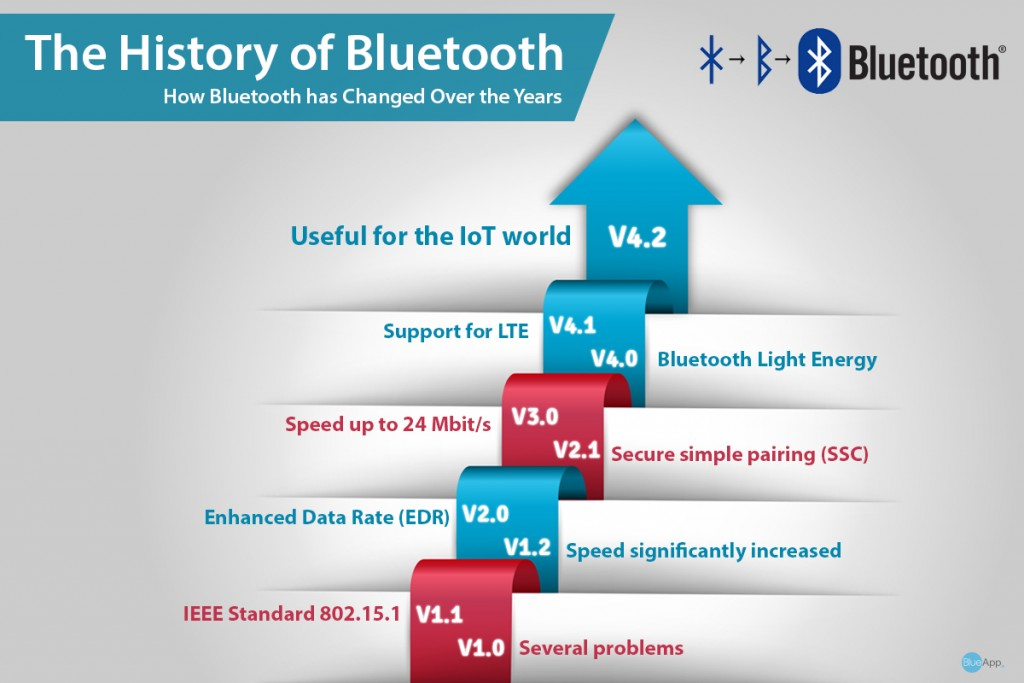
\includegraphics[width=15cm,height=8cm]{history.jpg}
    \caption{Evolution of Bluetooth}
    \end{figure}
	 {Bluetooth is named after King Harald Bluetooth. He united several Danish tribes (now present day Denmark, Sweden, and Norway) into a single kingdom. and may have also introduced Christianity as well. Jim Kardach was the man who proposed the idea of naming this system after King Bluetooth. A system was developed as a way for mobile phones to communicate with computers. It is implied that Bluetooth unites communication protocols into one universal standard, just like King Bluetooth united Danish tribes.
	 The technique that Bluetooth bases its communication protocol on is accredited to patent from 1942. The technique used by Bluetooth is called frequency hopping spread spectrum or FHSS. The patent was issued for a radio controlled torpedo and was called “Secret Communication System”. This was developed so enemies could not jam a signal during World War II. However, the US Navy did not end up using this technique, but it has become very useful for us today.

Bluetooth Special Interest Group (SIG)

In 1994, Ericsson, a communication and services company, had the idea of replacing RS-232 cables with a wireless system. In addition, other companies like Nokia, Intel, Toshiba, and IBM had similar ideas to make a wireless communication protocol for mobile phones and computers. These companies met in an Ericsson plant in Sweden to finalize the formation of the Bluetooth SIG in 1996. These companies realized that they needed to work together in order to make a universal standard.

This meeting is apparently where Kardach came up with the name for Bluetooth. This name was only to be used for a short period of time until a better name was thought of, but obviously, that never happened. As of today, Bluetooth devices have surpassed 2.5 billion and membership in the Bluetooth SIG has increased to over 19,000 from the initial 5 companies. This trend does not seem to be slowing down anytime soon.

Today, The Bluetooth SIG headquarters is in Kirkland, Washington. There are also offices in Hong Kong, Beijing, Seoul, Minato-Ku, Tokyo, Taiwan, and Malmo.

The Bluetooth SIG performs many functions such as updating Bluetooth specifications and protecting the trademark for Bluetooth. For a detailed timeline of the Bluetooth SIG, go here.

Different Versions of Bluetooth:
\begin{itemize}

\item Bluetooth v1.0: This version had several problems and did not work very well with other devices. It also required a Bluetooth hardware device address while connecting to other devices causing many problems.

\item Bluetooth v1.1: In 2002, this was under the name IEEE Standard 802.15.1. This version fixed many of the errors in the past version. It also added a Signal Strength Indicator and non-encrypted channels were now available.

\item Bluetooth v1.2: This was a huge improvement from version 1.1. For example, the connection and discovery speed was significantly increased.

\item Bluetooth v2.0: Released in 2004, this version used Enhanced Data Rate (EDR) to help improve data transfer rate. EDR also uses less power solving some of the problems of the past versions.

\item Bluetooth v2.1: This version came out in 2007. This version main improvement was the use of secure simple pairing (SSC). With this, device pairing became more efficient and security was improved.

\item Bluetooth v3.0: In 2009, this version was released with improved transfer speeds of up to 24 Mbit/s. This was due to Alternative MAC/PHY (AMP).

\item Bluetooth v4.0: This version came out in 2010. This was the version where Bluetooth Light Energy or BLE came out. This has been used more and more due to its energy saving capabilities and speed of data transfer.

\item Bluetooth v4.1: One year after 4.0, v4.1 came out in 2013. This update was a major software update. This included support for LTE.

\item Bluetooth v4.2: One year later, 4.2 came out in 2014 and made it more useful for the IoT world.

\end{itemize}
In 2016, Bluetooth is planning on improving even more making it faster and giving it a longer range. Bluetooth has been a big part of our lives and hopefully this article helped you understand how it came to be in its current state.
}

    \newpage
	\section{BLE Specifications}
	Difference between Classical Bluetooth and BLE.
	\begin{figure}[h]
    \centering
    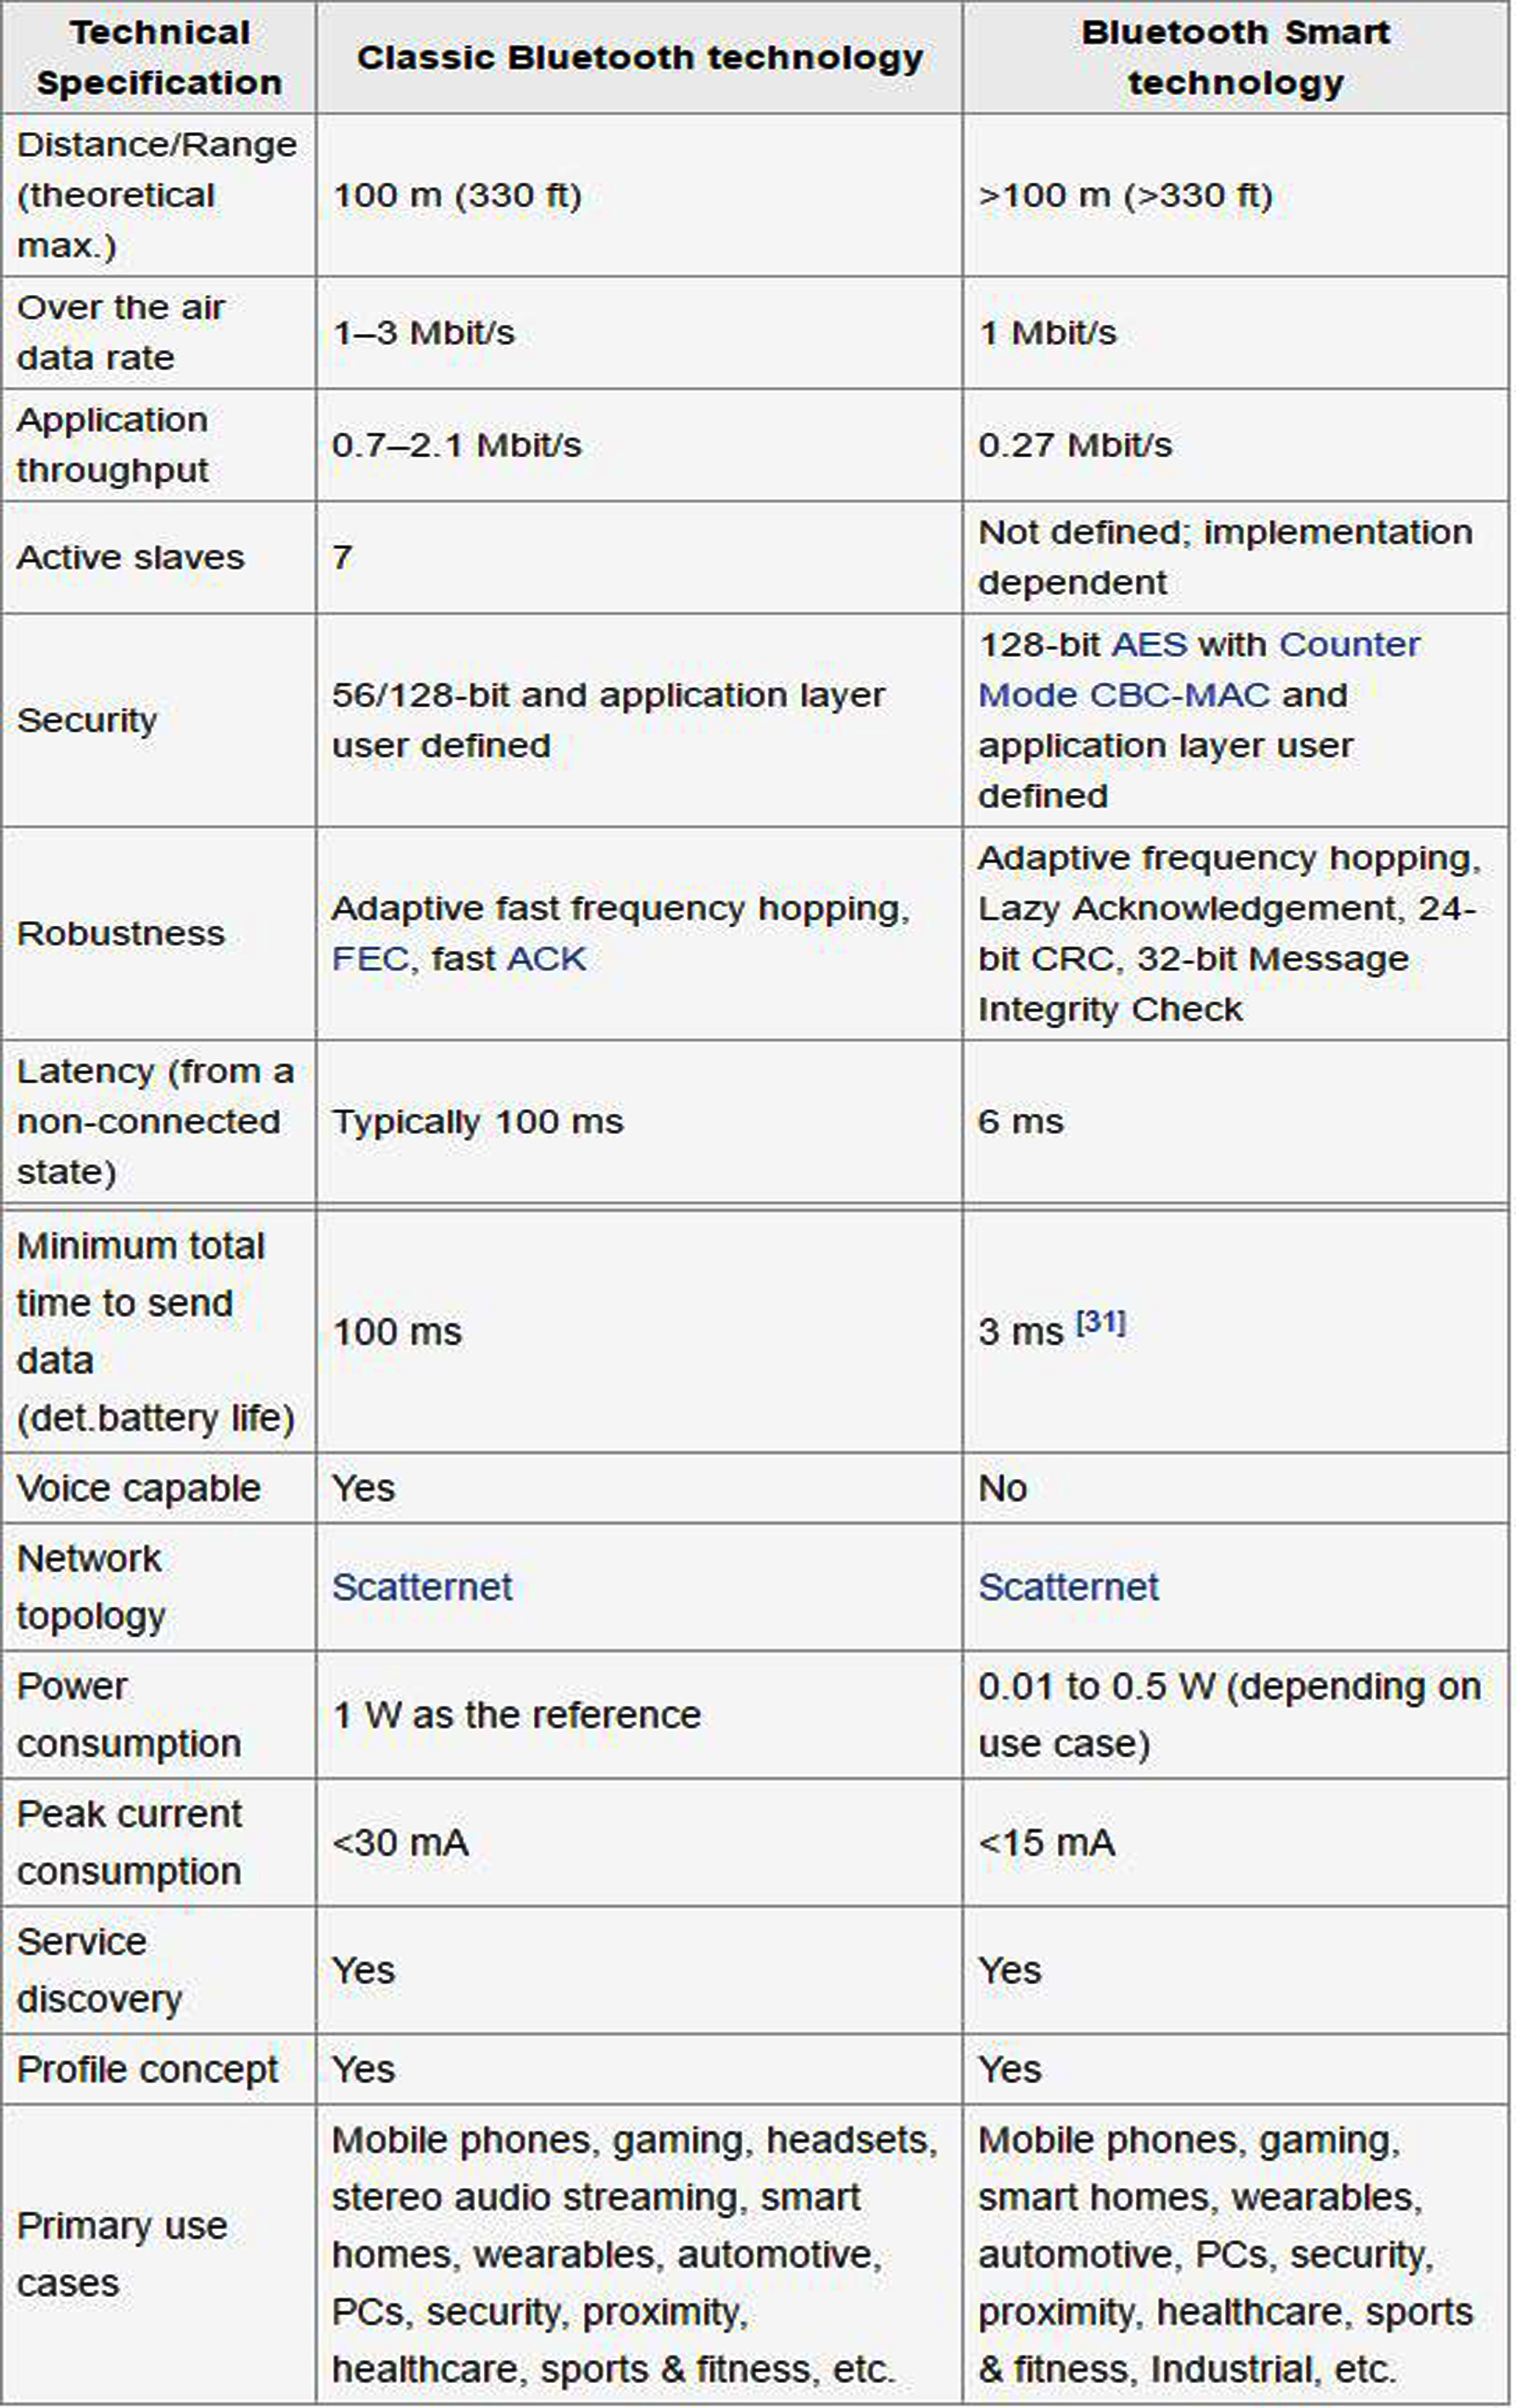
\includegraphics[width=10cm,height=15cm]{table.jpg}
    \caption{BLE Specifications}
    \end{figure}
	
	  \newpage
	\section{Why low energy is important ?}
	{
Due to its inexpensive and energy efficient properties, Bluetooth Low Energy is ideal for IoT devices that rely on the constant collection of data. BLE has given developers the ability to make leaps and bounds when developing for wearable technology and devices that can be controlled remotely or via mobile devices. Developers in the consumer electronic and internet-connected (IoT) machine industries utilize Bluetooth Low Energy technology not only due to its low cost and long battery life, but also due to its ease of deployment into existing appliances and compatibility with current technology. From health monitors to smart watches and fitness trackers, Bluetooth LE can use a dime-sized battery for up to a year to send short-range wireless data.

For developers, this means creating technology that takes advantage of 24-7 data collection, extremely low energy requirements, and wireless communications in an inexpensive, flexible environment.
	}
	
	\newpage
	\section{Ble's place in crowd}
	{
	Bluetooth was considered to be in the Wi-Fi camp due to such factors as standardized data transfer with fairly high-power consumption. In its original release, Bluetooth supported 1Mbit/sec data transfer (Bluetooth 1.2). Since then, this number was increased to 3Mbit/sec with an Enhanced Data Rate version (Bluetooth 2.0 + EDR), and even further with a High-Speed version, Bluetooth 3.0 + HS. Now Bluetooth 4.0 moves to the other end of the spectrum targeting lower power, small size of data transfer with low duty cycle types of applications.

A place for BLE does exist, but it may not be easy to identify. BLE is intended for light duty cycle devices that support small data throughput and operate a long time on a coin-sized battery. Such wireless connectivity comes with a minimal price (inexpensive silicon, light MCU processing requirements, reduced memory footprint), and it can be used in applications related to the Body Area Network (BAN) which represents a connectivity bubble that moves along with the individual.  After putting all requirements together it is easy to see that none of existing wireless solutions is a good fit in this case.

Let's first eliminate candidates that require a rechargeable battery or are capable of supporting streaming data--no Wi-Fi. The primary candidate for this job is an 802.15.4 based network and it has such multiple variations as ZigBee, 6LoWPAN, etc. In general, however, the average power consumption for a ZigBee node is in the range of 30ma, which is above the capacity of a coin cell battery.

 

Given that a ZigBee network with a 30ma power consumption budget allows nodes to be placed within a range of 100 feet, BLE is designed to work within a 30-foot range. BLE use cases circle around the user and their immediate surroundings. Since all devices are within a reachable distance, no retransmission using an intermediate node is required. It not only provides a cut in power consumption but also reduces network organization to a simple star type of connectivity.

 

It is fair to say that BLE has a respectable contestant from the camp of proprietary wireless technologies, the ANT protocol. Used with a Nordic ultra low power SoC, it operates within a required power budget and it has a compelling use case: ANT is used in Garmin devices that communicate with pedometers and other sport related products [2].

 

But, here is a rocket booster for BLE--under the Bluetooth umbrella, BLE is not only standardized, but will also inhabit over 2 billion cell phones, which will have regular Bluetooth and it smaller brother, Bluetooth LE.

 

Again, although it would rather artificially limit the BLE area of application, let+s state that BLE is optimized to enable wireless communication between a smart phone and low data rate, coin battery operated, potentially disposable device located in a close vicinity. On the top of that, let+s assume that BLE functionality comes virtually free and is already built into the cell phone as an addition to regular Bluetooth. Within this paradigm, BLE has an unbeatable stronghold against other contenders.
	}
	
	
	
	    \newpage
		\section{GATT}
		\subsection{Introduction }
	{
    GATT is an acronym for the Generic Attribute Profile, and it defines the way that two Bluetooth Low Energy devices transfer data back and forth using concepts called Services and Characteristics. It makes use of a generic data protocol called the Attribute Protocol (ATT), which is used to store Services, Characteristics and related data in a simple lookup table using 16-bit IDs for each entry in the table.

GATT comes into play once a dedicated connection is established between two devices, meaning that you have already gone through the advertising process governed by GAP.

The most important thing to keep in mind with GATT and connections is that connections are exclusive. What is meant by that is that a BLE peripheral can only be connected to one central device (a mobile phone, etc.) at a time! As soon as a peripheral connects to a central device, it will stop advertising itself and other devices will no longer be able to see it or connect to it until the existing connection is broken.

Establishing a connection is also the only way to allow two way communication, where the central device can send meaningful data to the peripheral and vice versa.
	}
	\newpage
	\subsection{GATT Transactions}
	\begin{figure}[h]
    \centering
    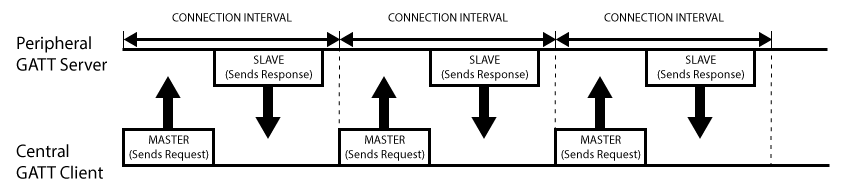
\includegraphics[width=11cm,height=4cm]{GattTransactions.png}
    \caption{Gatt Master-Slave Transactions}
    \end{figure}
	{An important concept to understand with GATT is the server/client relationship.

The peripheral is known as the GATT Server, which holds the ATT lookup data and service and characteristic definitions, and the GATT Client (the phone/tablet), which sends requests to this server.

All transactions are started by the master device, the GATT Client, which receives response from the slave device, the GATT Server.

When establishing a connection, the peripheral will suggest a 'Connection Interval' to the central device, and the central device will try to reconnect every connection interval to see if any new data is available, etc. It's important to keep in mind that this connection interval is really just a suggestion, though! Your central device may not be able to honour the request because it's busy talking to another peripheral or the required system resources just aren't available.

The following diagram should illustrate to data exchange process between a peripheral (the GATT Server) and a central device (the GATT Client), with the master device initiating every transaction:}

    \newpage
	\section{Applications}
	{
    All current low energy application profiles are based on the generic attribute profile (GATT).The Bluetooth SIG recently formed the Smart Mesh study group to research and define its use cases in an effort to define a standard specification.
    \begin{itemize}
 \item   Health care profiles
There are many profiles for Bluetooth Smart devices in healthcare applications.
\begin{itemize}
\item BLP (Blood Pressure Profile)— for blood pressure measurement.
\item HTP (Health Thermometer Profile) — for medical temperature measurement devices.
\item GLP (Glucose Profile) — for blood glucose monitors.
\item CGMP (Continuous Glucose Monitor Profile)
\end{itemize}
\item Sports and fitness profiles
Profiles for sporting and fitness accessories include:
\begin{itemize}
\item BCS (Body Composition Service)
\item CSCP (Cycling Speed and Cadence Profile) — for sensors attached to a bicycle or exercise bike to measure cadence and wheel speed.
\item CPP (Cycling Power Profile)
\item HRP (Heart Rate Profile) — for devices which measure heart rate
\item LNP (Location and Navigation Profile)
\item RSCP (Running Speed and Cadence Profile)
\item WSP (Weight Scale Profile)
\end{itemize}
\begin{itemize}
\item Internet Connectivity
\item IPSP (Internet Protocol Support Profile)
\end{itemize}
\begin{itemize}
\item Generic Sensors
\item ESP (Environmental Sensing Profile)
\item UDS (User Data Service)
\end{itemize}
\begin{itemize}
\item HID Connectivity
\item HOGP (HID over GATT Profile)
\end{itemize}
\item Proximity sensing\\
"Electronic leash" applications are well suited to the long battery life possible for 'always-on' devices.[20] Manufacturers of iBeacon devices implement the appropriate specifications for their device to make use of proximity sensing capabilities supported by Apple Inc. compatible iDevices.

\item Relevant application profiles:
\begin{itemize}
\item FMP — the "find me" profile — allows one device to issue an alert on a second misplaced device.[22]
\item PXP — the proximity profile — allows a proximity monitor to detect whether a proximity reporter is within a close range. Physical proximity can be estimated using the radio receiver's RSSI value, although this does not have absolute calibration of distances. Typically, an alarm may be sounded when the distance between the devices exceeds a set threshold.
\end{itemize}
\item Alerts and time profiles\\
The phone alert status profile and alert notification profile allow a client device to receive notifications such as incoming call alerts from another device.
The time profile allows current time and time zone information on a client device to be set from a server device, such as between a wristwatch and a mobile phone's network time.
\item Battery\\
The Battery Service exposes the Battery State and Battery Level of a single battery or set of batteries in a device.
\end{itemize}
	}
    \newpage
	\section{ References}
	{
	http://www.edn-europe.com/blog/bluetooth-low-energy-ble-short-history-ble-standard-and-gatt\\
	http://www.zymo.io/bluetooth-low-energy/\\
	https://en.wikipedia.org/wiki/Bluetooth_low_energy\\
	https://www.bluetooth.com/media/our-history\\
	}

	
\end{document}
